\documentclass[11pt, a4paper]{report}

\usepackage[T1]{fontenc}
\usepackage[utf8]{inputenc}
\usepackage[english]{babel}
\usepackage[top=3cm, bottom=3cm, left=2cm, right=2cm]{geometry}
\usepackage{graphics}
\usepackage{graphicx}
\usepackage{eurosym}
\usepackage{soul}
\usepackage{graphicx}
\usepackage{amsmath}
\usepackage{relsize}
\usepackage{titlepic}
\usepackage{tocloft}


\renewcommand\cftchapfont{\LARGE\bfseries}
\renewcommand\cftsecfont{\Large}

\renewcommand\cftchapafterpnum{\par\addvspace{10pt}}
\renewcommand\cftsecafterpnum{\par\addvspace{6pt}}



\begin{titlepage}
\newcommand*{\defeq}{\stackrel{\mathsmaller{\mathsf{def}}}{=}}
\title{English project:\\Words and the World}
\author{Gauthier ZAMBAUX and Nicolas DUBOIS}
\date{\today}
\titlepic{
\includegraphics[scale=0.5]{images/telecomnancy.png}

\includegraphics[scale=1]{images/universitelorraine.jpg}}
\end{titlepage}





\begin{document}

\maketitle


\chapter*{Introduction}
\addcontentsline{toc}{chapter}{Introduction}
\paragraph{}This report introduces the reader to an application that we have been developping as part of the English Module of TELECOM Nancy. This application aims at helping its users learn about the English language and its history.

\paragraph{}The \textit{Words and the World} application was created after realizing that learners of English are often not very well familiar with both dialectal differences and the history of the language. Both being closely related we have decided to design a software that allows the user to work on those two things in order with the goal to help them improve their knowledge of English-speaking countries and their understanding of different accents and slangs.

\paragraph{}As a consequence, the application is devided into two parts, one that allows the user to learn slang words and idioms from various English-speaking countries and another that deals with the spread of the British Empire throughout the world, and therefore of the English language. Indeed, the English language has evolved a lot following different paths over the past centuries that it has been spoken in various regions around the world.

\paragraph{}This report is a presentation of the \textit{Words and the World} application. It will first introduce a user documentation written in English and then a technical documentation in French.

\newpage
\tableofcontents
\newpage


\chapter*{User Documentation}
\addcontentsline{toc}{chapter}{User Documentation}
\paragraph{}The \textit{Words and the World} application was designed to help you learn more about differences between English dialects in various countries and the history of the British empire. It is thus devided into two distinct parts that are however related in that they both deal with the spread of the English language around the world. This software was designed to be usable on most computer operating systems that can support Java applications and does not reaquire a connection to the Internet to work.

\paragraph{}After launching the application, the user is presented with the home tab where they can find a brief desciption of the software and links to the language (about dialectal differences in English) and history (about the history of the British Empire) tabs. This main page is however not accessible anymore once they have chosen a tab as they can easily navigate directly between the history and the language tabs.

\section*{The history of the British empire}
\addcontentsline{toc}{section}{The history of the British empire}
\paragraph{}The first tab of the application is designed to teach the user about the history of the spread of the British empire. When the user clicks on the history tab button, they are presented with a description of what they can find in this part of the app. This tab is designed as a history course split in an number of pages describing each a moment of that history, using maps to emphasize the information and help the user remember through visual stimulation.

\paragraph{}In the following pages is described the creation of the major British colonies, along with their end and the creation of the Commonwealth. The user can navigate between the different pages using the "prvious" and "next" arrows.

\paragraph{}The application describes the major events of the colonisation conducted by the British Crown since the seventeenth century, starting from the first settlements of the Americas up to the decolonisation of Hong-Kong.

\paragraph{}For each event described the user is presented with a picture, usually a map, and a short text summurising important facts.

\paragraph{}Most of the events or organised in chronological order with some events ovelapping.



\section*{How English is English?}
\addcontentsline{toc}{section}{How English is English?}
\paragraph{}This part of the application allows the user to discover differences in words and expressions between several dialects of English. Indeed the English language has the caracteristic to easily absorb vocabulary from other languages, and this feature has brought to the emergence of a variety of different kinds of English around the world.

\paragraph{}The first page the user is presented to when checking the language tab shows a map of the world with the names of the countries supported by the app. As of today the database of the software support five countries that are the United States of America, the United Kingdom, South Africa, India and Australia, and each of those countries is accompanied by around fifty words. Any user or teacher can supplement the database easily by only adding words to the database file; however adding new countries requires modifying the source code of the programme. To access a certain country's vocabulary, the user needs to click on its name.

\vspace{0.15cm}
\centerline{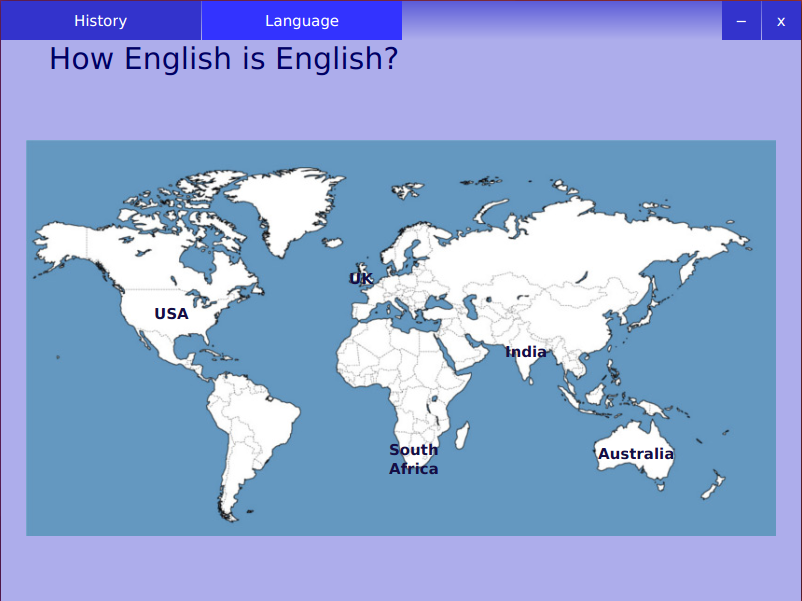
\includegraphics[scale=0.5]{images/languageTab.png}}

\paragraph{}For each country, the user can discover a variety of vocabulary words and idioms with definition in standard English and an example. The word that is presented to them is chosen randomly in the database and the software avoids presenting twice the same word in a row.

\paragraph{}For each word, the play button allows the user to listen to the expression as it is pronounced using the native country's pronunciation.

\vspace{0.2cm}
\centerline{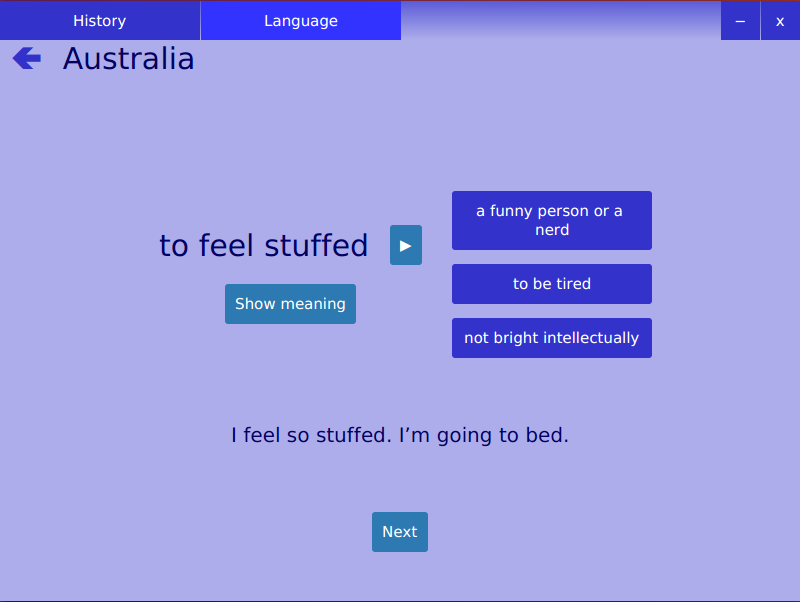
\includegraphics[scale=0.5]{images/AustraliaQuestion.png}}
\vspace{-0.35cm}

\paragraph{}They can also test their knowledge with a multiple choice test as the definition of a word does not appear unless the user wants to. The answers of the test are not memorized by the application and the user can test their knowledge of a word an infinite number of times.

\vspace{0.08cm}
\centerline{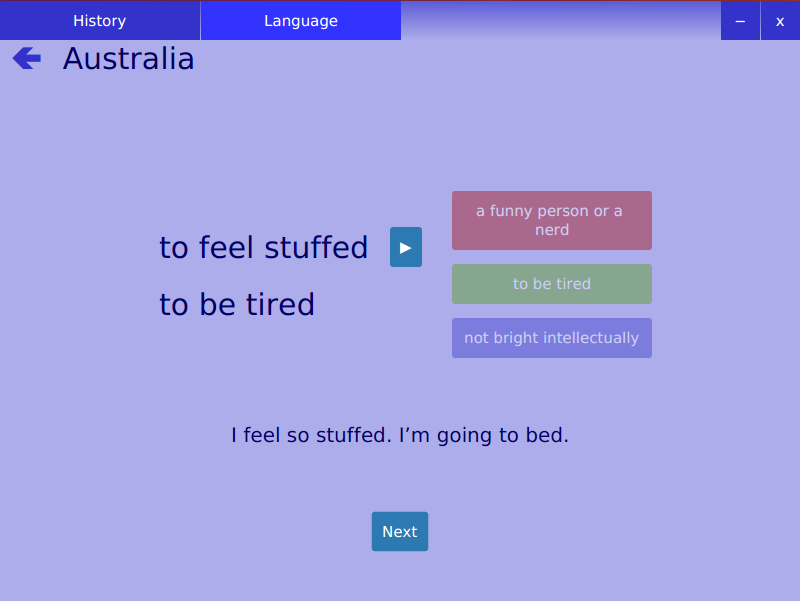
\includegraphics[scale=0.5]{images/AustraliaWrongAnswer.png}}



\chapter*{Technical documentation}
\addcontentsline{toc}{chapter}{Technical documentation}
\paragraph{}Parce que nous maîtrisions ce langage et de manière à pouvoir produire une application intéressante, nous avons choisi d'utiliser le langage de programation \textit{Java}. En plus de nous être familier, ce langage est puissant et multiplateforme puisqu'un programme écrit en Java peut fonctionner sur n'importe quel ordinateur équipé du logiciel éponyme d'\textit{Oracle}. Le \textit{Java} est par ailleurs très répendant dans le développement d'applications professionnelle et son choix pour ce projet nous a donné une occasion supplémentaire de le pratiquer.

\paragraph{}Pour ce qui est de l'interface graphique de l'application, nous avons choisi de nous tourner vers la bibliothèque graphique \textit{JavaFX} qui, avec \textit{Swing} (une autre bibliothèque graphique du langage \textit{Java}), est standard. L'utilisation de cette bibliothèque plutôt que \textit{Swing} par exemple était à la fois un défi puisqu'elle est parfois moins intuitive à utiliser, mais aussi un atout puisqu'elle permet une plus grande flexibilité sur le plan graphique.

\paragraph{}En effet, en plus des fonctions et classes natives que comprend \textit{JavaFX} qui permettent déjà une grande possibilité de personnalisation d'interfaces, la bibliothèque peut être utilisée en concert avec le langage de style \textit{CSS} (\textit{Cascading Style Sheets}). Ce langage, originellement créé pour le style de page internet et généralement utilisé avec le \textit{HTML} (\textit{HyperText Markup Language}) qui est un langage de description de pages internet. Le langage \textit{CSS} permet notamment de définir les couleurs, les polices de caractère, la position des objets et leur tailles, les contours ou encore les images de fond. Il nous a été particulièrement utile pour des détails de la présentation des informations par exemple pour le positionnement des titres.

\paragraph{}Nous nous sommes efforcé pour ce ce projet de développer une interface graphique agréable et intuitive. Nous avons notamment choisi des couleurs cohérentes et placé les différents éléments des pages de façon ludique. Par ailleurs, pour éviter des déplacements d'objets peut souhaitables dasn les pages, nous avons interdit le redimensionnement de la fenêtre.

\paragraph{}En plus de \textit{JavaFX} pour l'interface graphique, nous avons dû trouver une source d'enregistrements audios correspondant aux accents des différents pays que nous avons choisis de représenter. Pour cela, nous avons eu recours à Google Translate qui permet en effet de choisir la prononciation du locuteur pour un enregistrement. Le téléchargement des fichiers audio s'est fait en lignes de commande par le biais du logiciel \textit{wget}. Nous avons choisi de télécharger l'intégralité des enregistrements nécessaires pour que l'application puisse être utilisée hors ligne.

\paragraph{}La lecture des enregistrements audios dans le logiciel a par ailleurs été un problème puisqu'il ne semble pas exister beaucoup de possiblités pour le faire, ou bien que les format d'enregistrements pris en charge de correspondaient pas à nos attentes car n'étant pas courant ou étant spécifiques à un système d'exploitation, notamment \textit{Windows}. Nous avons finalement trouvé la bibliothèque \textit{JLayer} qui se spécialise dans le décodage et la lecture de fichiers \textit{MPEG}/\textit{MP3}. Bien que cette bibliothèque soit ancienne et plus mis à jour depuis plusieurs années, elle ne nous a pas posé de problème et est facile à mettre en place et utiliser.

\paragraph{}Nous nous sommes aussi beaucoup interrogés pour ce qui est de la construction de la base de données des mots pour chaque pays. En effet, nous pensions au début utiliser une base de données de type \textit{MySQL} à compléter en lignes de commandes. Cependant, nous avons eu quelques problèmes de mise en place de la base. Bien qu'il nous était sans problème possible de créer les tables de la base de données et de les remplir, nous ne pouvions pas récupérer le fichier résultant par la suite. Ne maîtrisant pas cette technologie, nous avons finalement décidé de revenir à un formatage des données plus classique avec un simple fichier \textit{CSV}. Ce type de fichier est simplement un fichier texte dans lequel chaque ligne correspond à une entrée de la base de données, et les données sont séparées par des points virgules (ou un autre symboles, comme une virgule simple).
Un autre avantage de ce type d'organisation des données est que ces fichiers peuvent être lus et modifier par un logiciel de type tableur classique (\textit{LibreOffice Calc} dans notre cas).

\vspace{0.5cm}
\centerline{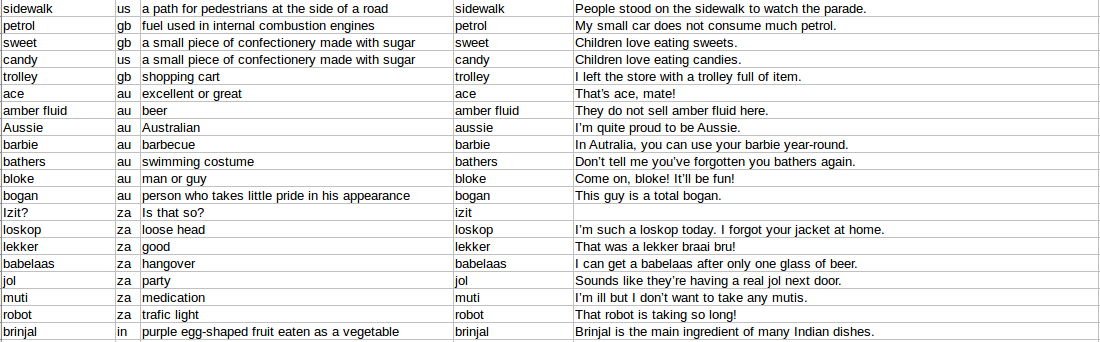
\includegraphics[scale=0.4]{images/database.png}}

\paragraph{}La capture d'écran ci-dessus montre une partie de la base de données. Les colonnes sont organisées dans l'ordre : mot, code pays, définition, nom du fichier audio correspondant, phrase d'exemple. Il apparaît ainsi qu'un avantage supplémentaire de ce type de fichiers est la personnalisation possible par l'utilisateur qui peut ajouter ou au contraire supprimer des mots. Remarquons tout de même que cela n'est possible que pour les pays déjà existant. Cette flexibilité peut notamment être utile pour un professeur qui voudrait utiliser l'application pour travailler le vocabulaire spécifique à un pays avec ses étudiants mais qui ne serait pas satisfait du contenu de la base de données existante.

\paragraph{}Pour ce qui est de la façon de  programmer, nous avons choisi d'organiser le code en suivant le modèle \textit{MVC} (Modèle, Vue, Controleur) qui consiste à séparer le code en trois parties, respectivement les données de l'application, l'interface graphique et les actions à effectuer. Ce type d'organisation du code dans un programme et particulièrement répendu et permet notamment à des spécialistes du graphisme de travailler en parallèle de personnes travaillant plutôt sur le contenu réel plutôt que sur l'affichage. Dans notre cas, cette façon d'organiser notre programme nous a permis de mieux nous organiser (du fait que l'on ait travaillé en équipe) et de mieux nous retrouver dans les différents fichiers du programme.

\paragraph{}Par ailleurs, le \textit{Java} est un langage purement orienté objet et il nous a donc fallu nous adapter aux contraintes liées à ce type de programation qui présente tout de même des avantages certains sur des langages impératifs comme le \textit{C} dans le cas d'interfaces graphiques particulièrement.

\paragraph{}Pour ce qui est de l'écriture du code à proprement parler, nous avons choisi d'utiliser l'environnement de développement (\textit{IDE}, Integrated Develipment Environment) \textit{Eclipse}, qui présente de nombreux avantages, comme celui de proposer de nombreuses fonctionnalités d'auto-complétion et de correction.

\paragraph{}De façon à pouvoir travailler en groupe et à distance, nous avons utilisé le logiciel de gestion \textit{git}, qui permet de partager du code et de travailler en même temps sur un programme. Nous nous sommes orienté naturellement vers ce logiciel car nous le maîtrisions et qu'il permet de travailler efficacement à plusieurs sur un projet.



\chapter*{Conclusion}
\addcontentsline{toc}{chapter}{Conclusion}
\paragraph{}Working on this project was something very interesting for us as it allowed us to work on a subject of out choice. Moreover it allowed us to improve our knowledge or several technologies such as
%nous a permis dapprendre des choses sur l'EB et du voc
%faits amusants pour le vocabulaire (kangooroo Au)


\chapter*{Appendix: Sources}
\addcontentsline{toc}{chapter}{Appendix: Sources}
\hspace{0.6cm}$blog.oxforddictionaries.com/2015/09/how-good-is-your-south-african-english/$\\

$www.koalanet.com.au/australian-slang.html$\\

$en.wikipedia.org/wiki/List\_of\_South\_African\_slang\_words$\\

$www.theguardian.com/commentisfree/2016/jan/04/indian-english-phrases-indianisms-english-americanisms-vocabulary$\\

$www.englisch-hilfen.de/en/words/be-ae2.htm$\\

$www.languageinindia.com/junjul2002/baldridgeindianenglish.html$\\

$www.brandsouthafrica.com/tourism-south-africa/travel/advice/saenglish$\\

$www.braai.co.za/blog/generalbraai/typical-south-african-words-and-their-meaning/$\\

$dictionary.cambridge.org/fr/$\\

$www.linguee.fr$\\

$fr.wikipedia.org/wiki/Empire\_britannique$\\

$fr.wikipedia.org/wiki/\%C3\%89volution\_territoriale\_du\_Royaume-Uni$\\

$www.the-map-as-history.com/demos/tome05/Map-of-the-British-Empire-european-colonization.php$\\

$drapeaufree.free.fr/COLONIESUK/coloniesuk.htm$\\

$www.1001fonts.com/cursive-fonts.html$\\

\end{document}